\section{Universal Smart Patient Health Record (USPHR)}

In any medical organisation, it is essential to keep a good organisation of the data about individual patients. Besides the usual requirements for this data, in terms of being easily accessible and well structured, new legislations such as GDPR put additional requirements in terms of the organisation, ownership, access and communication of this data. The data is owned by the patient themselves and they need to be able to have full access to it, while the other parties (general practicioners, specialists, insurers) must have access to only the parts of the data that are releveant to diagnostics, treatment and insurance. Currently, there is no unified way to represent the patient data across different organisations. Each individual organisation (e.g.~National Health Service in the UK) might have their own way of organising the data. Quite frequently, this data is not even in the electronic format. This effectively prevents developing any generic mechanisms for storing, communicating and analysing the medical data, as each solution is tied up to a specific format of the data that is used by a particular organisation.

Universal Smart Patient Health Record (USPHR) represents a first attempt of a unified mechanism to create and manage electronic patient records for individual patients in a secure and transparent way, centralising a golden source of health information. It will overcome the current challenges arising from managing different formats of the diverse electronic patient records present in different institutions/scenarios by creating a universal format that will be applicable in a variety of situations. We have the following requirements for the format of USPHR:

\begin{itemize}
\item it needs to be \emph{general} enough so that it can encapsulate different use cases in the \textbf{Serums} project and wider;
  \item it needs to be \emph{specific} enough that it allows generation of machine-readable metadata that can be used for data fabrication and other parts of the \textbf{Serums} infrastructure;
  \item it needs to be \emph{flexible} enough to allow different levels of access by different interested parties, as well as the usage of blockchain to record lineage and provenance of the data;
\end{itemize}

\noindent
The USPHR will provide a fundamental core structure for the mechanisms from WP3, WP4, and WP5.


\section{General Data Vault}

\subsection{What is a Data Vault?}
\label{sec:datavault}

Data vault modelling is a database modelling methodology design that provide long-term historical storage of data coming in from multiple operational systems.
%
The base design principal is single version of the truth (SVOT) that supports data warehousing for either a single centralised database or a distributed synchronised database. This method is accomodating of change. Its adaptability provides resilience over time to changes in the data and data structures.
%
The data vault methodology is based on SEI/CMMI Level 5 best practices.
\\
\noindent
This is an example of a data vault:

\begin{figure}[H]
    \centering
    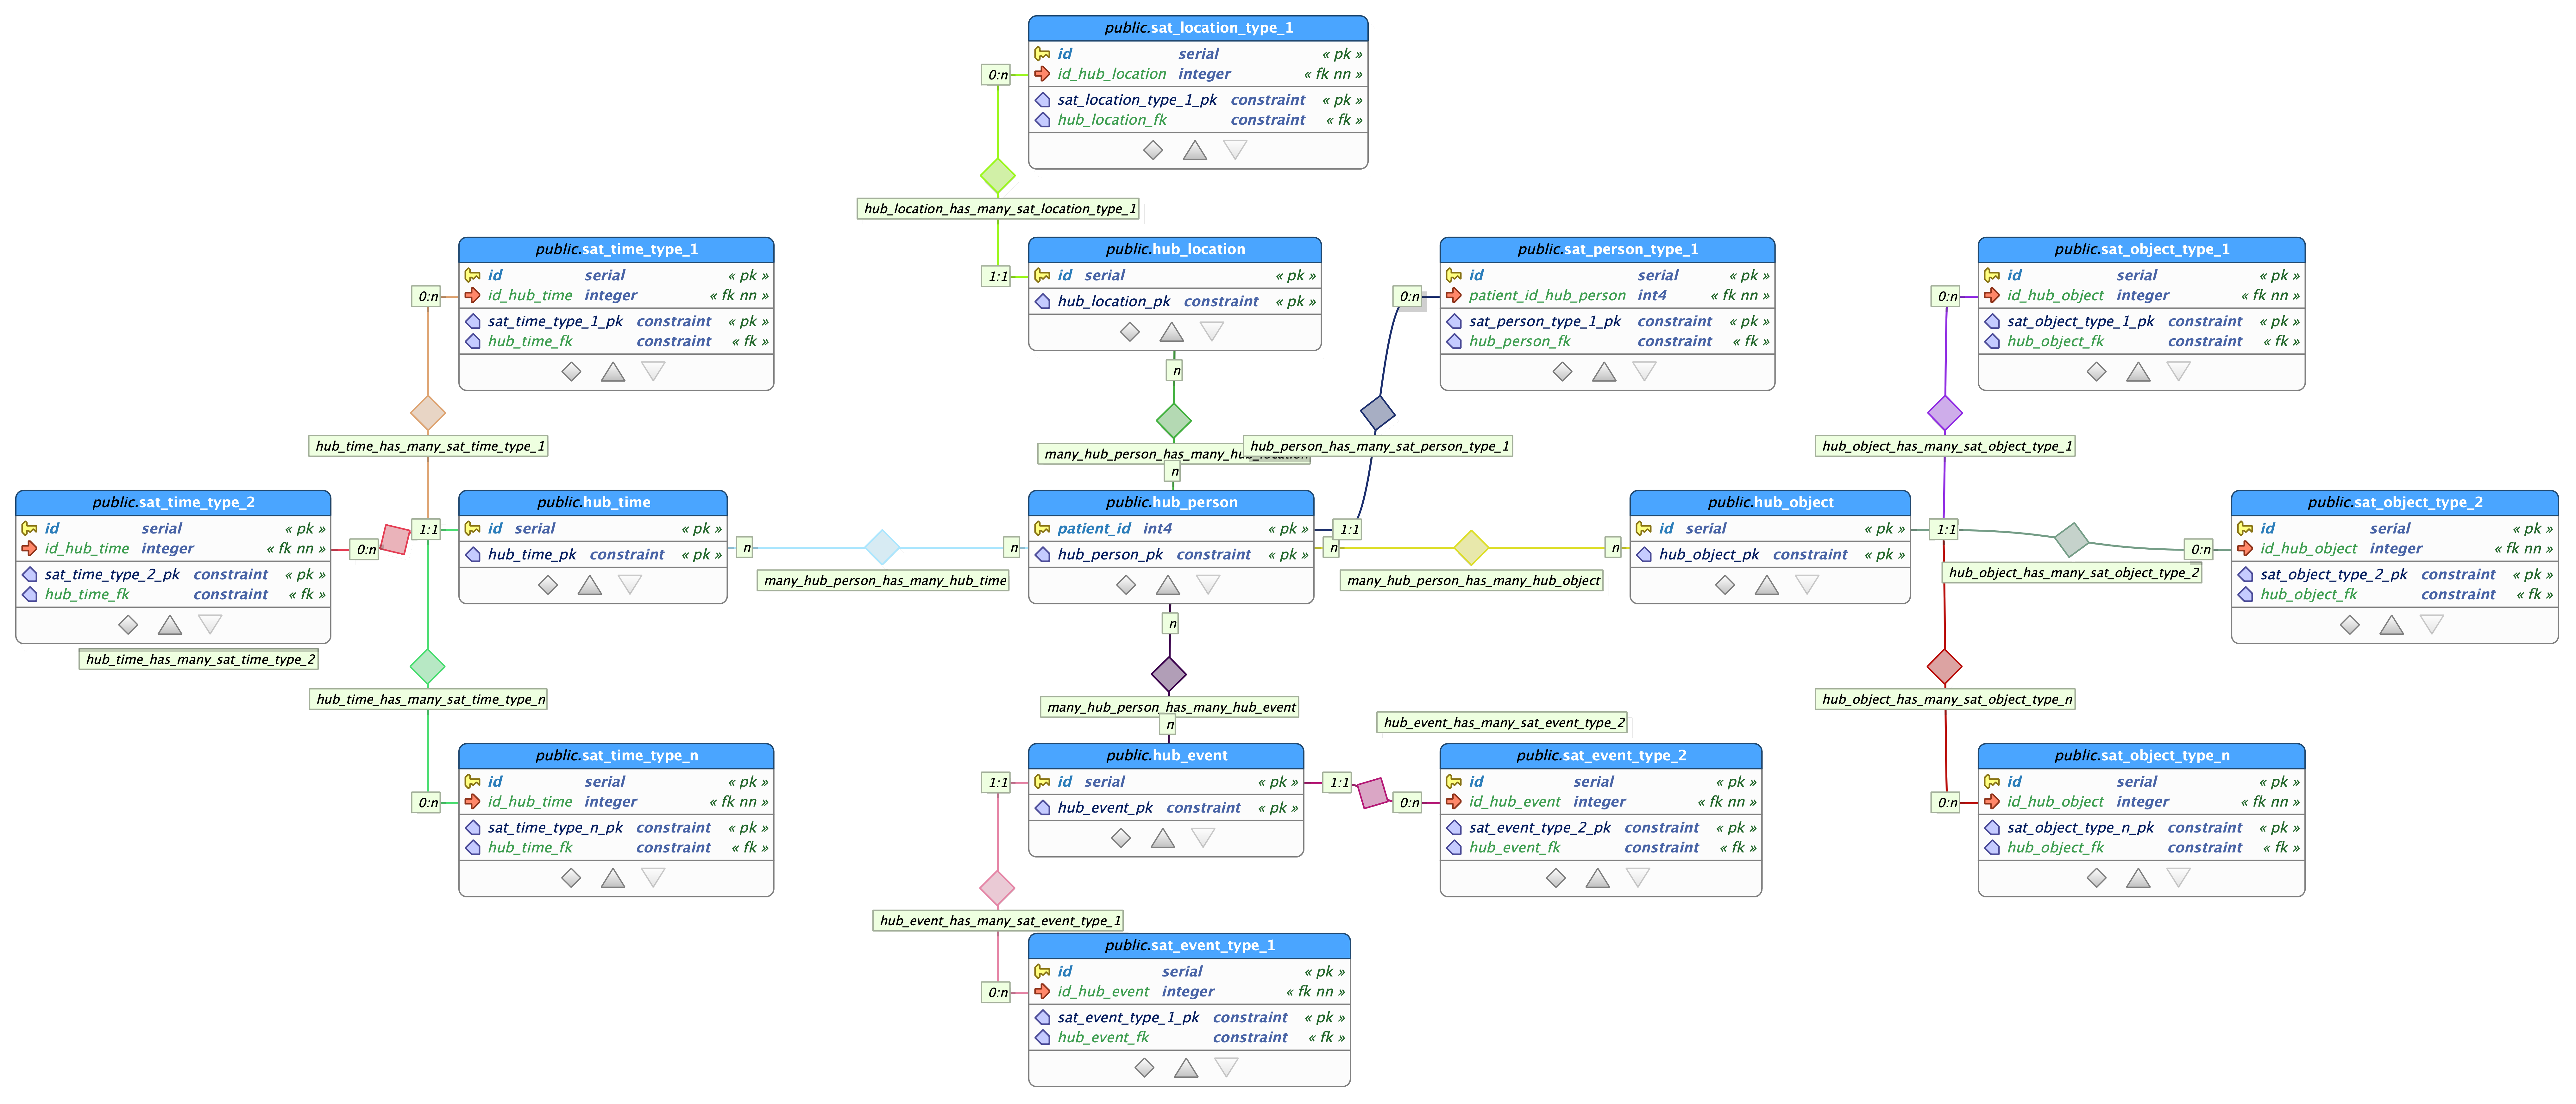
\includegraphics[width=10cm]{figures/technical/universal_smart_patient_record.png}
    \caption{Data Vault - Universal Smart Patient Health Record}
    \label{fig:dvlinks}
\end{figure}

The data vault model is comprised of three different types of tables:

%\section{Hubs, Links and Satellites}

%\subsection{Hubs}
\begin{itemize}
\item \emph{hubs}, that contain a list of unique business keys with low propensity to change;

\begin{figure}[H]
    \centering
    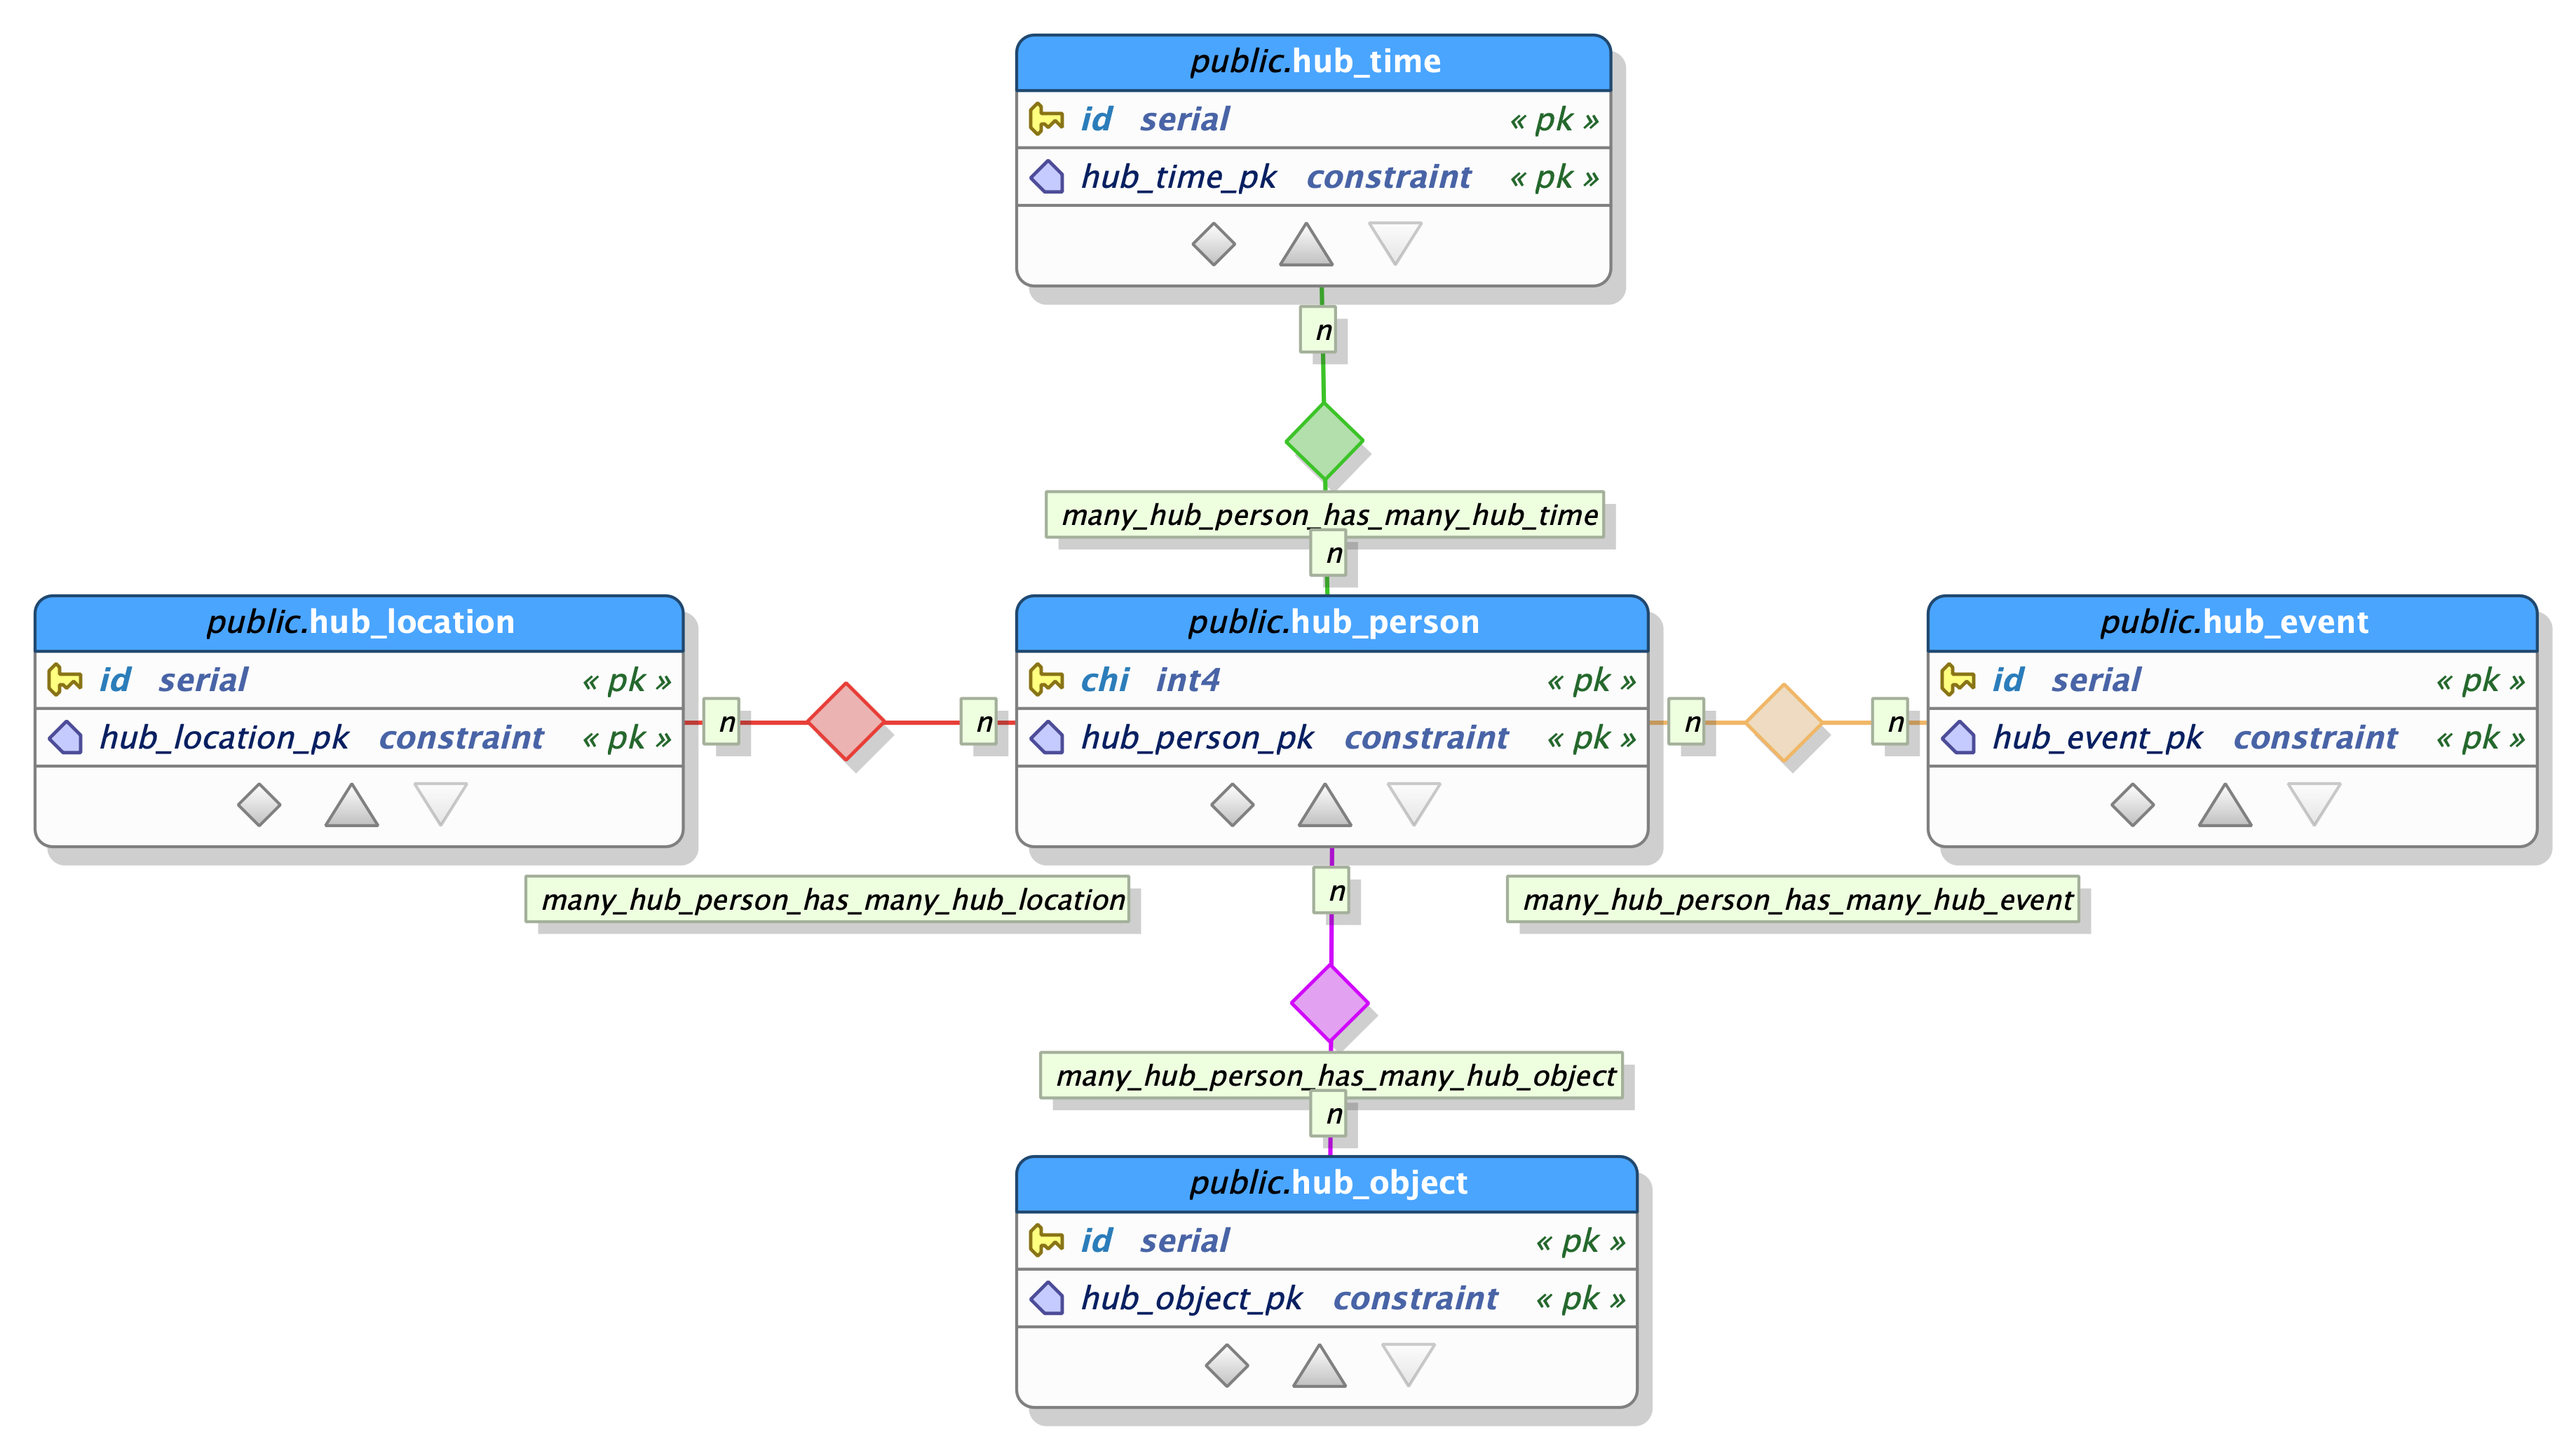
\includegraphics[width=10cm]{figures/technical/tpole_hubs.png}
    \caption{Data Vault - T-P-O-L-E Hubs}
    \label{fig:dvhubs}
\end{figure}

\item \emph{links} that represent associations or transactions between business keys (Hubs);

\begin{figure}[H]
    \centering
    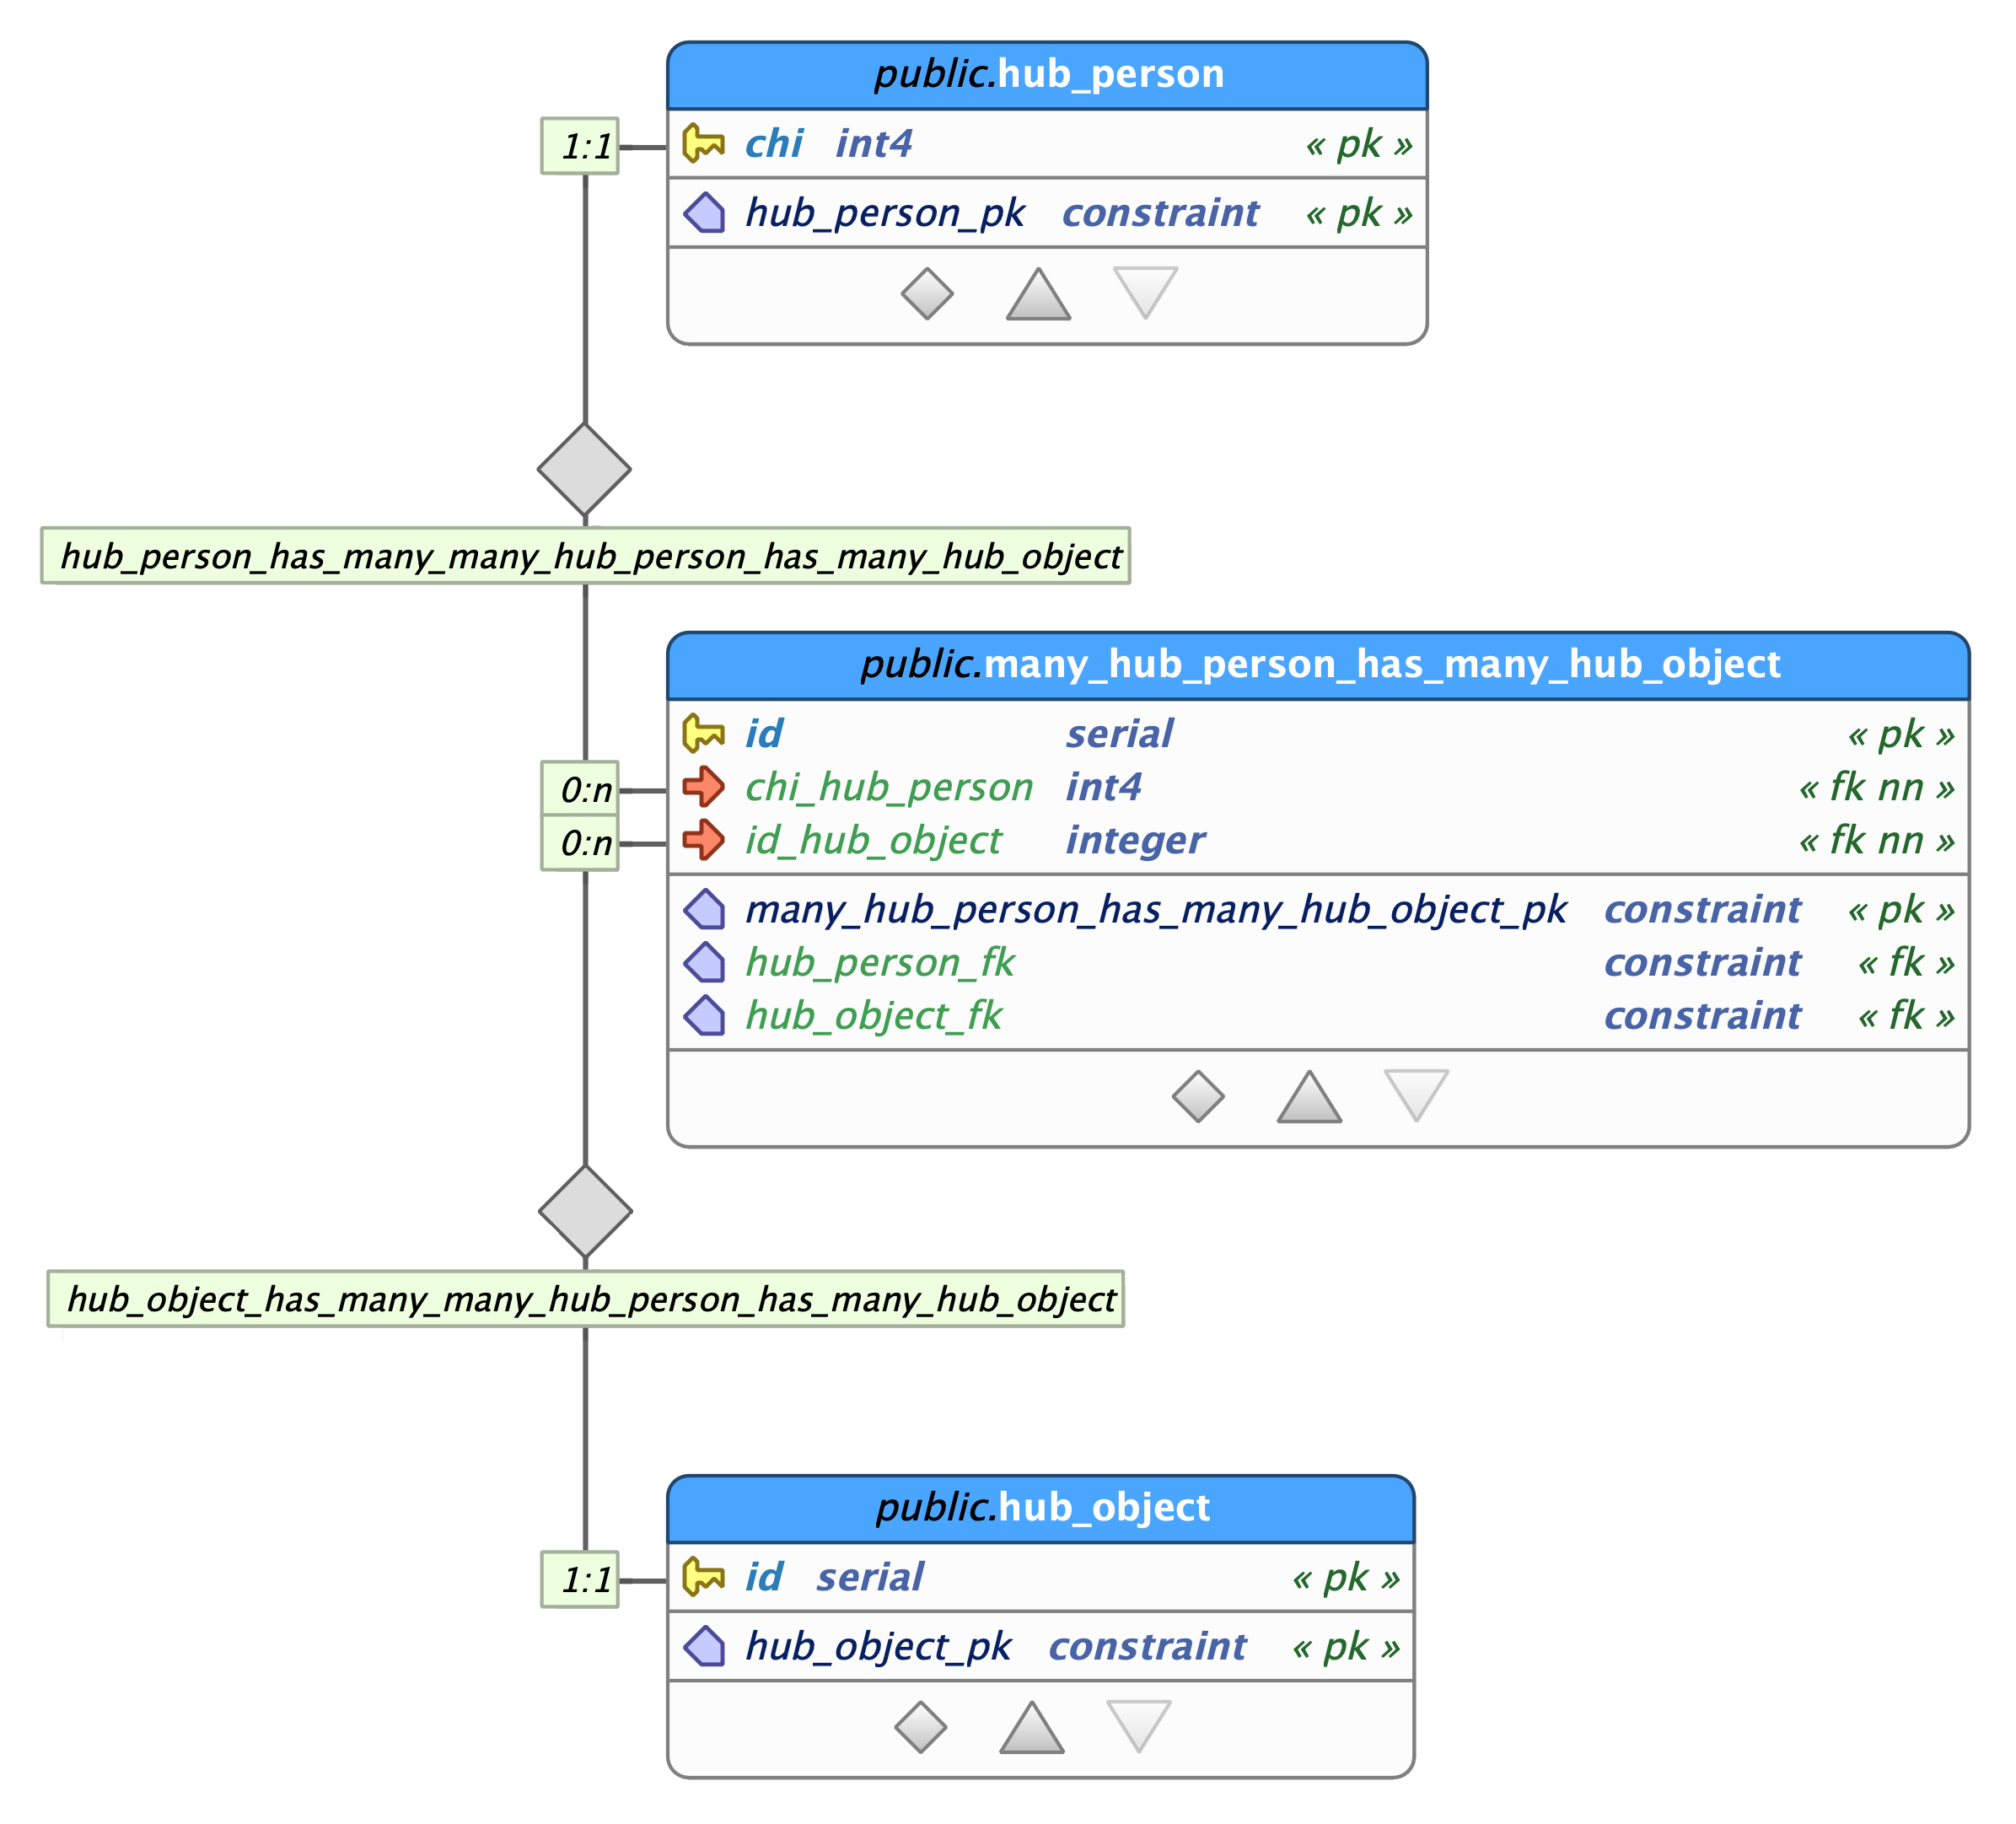
\includegraphics[width=10cm]{figures/technical/links.png}
    \caption{Data Vault - T-P-O-L-E Links}
    \label{fig:dvlinks}
\end{figure}

\item \emph{satellites}, where temporal and descriptive attributes of the hubs and links are stored;

%The hubs and links form the structure of the model, but holds neither temporal attributes nor descriptive attributes. These attributes are stored in separate tables called satellites.

\begin{figure}[H]
    \centering
    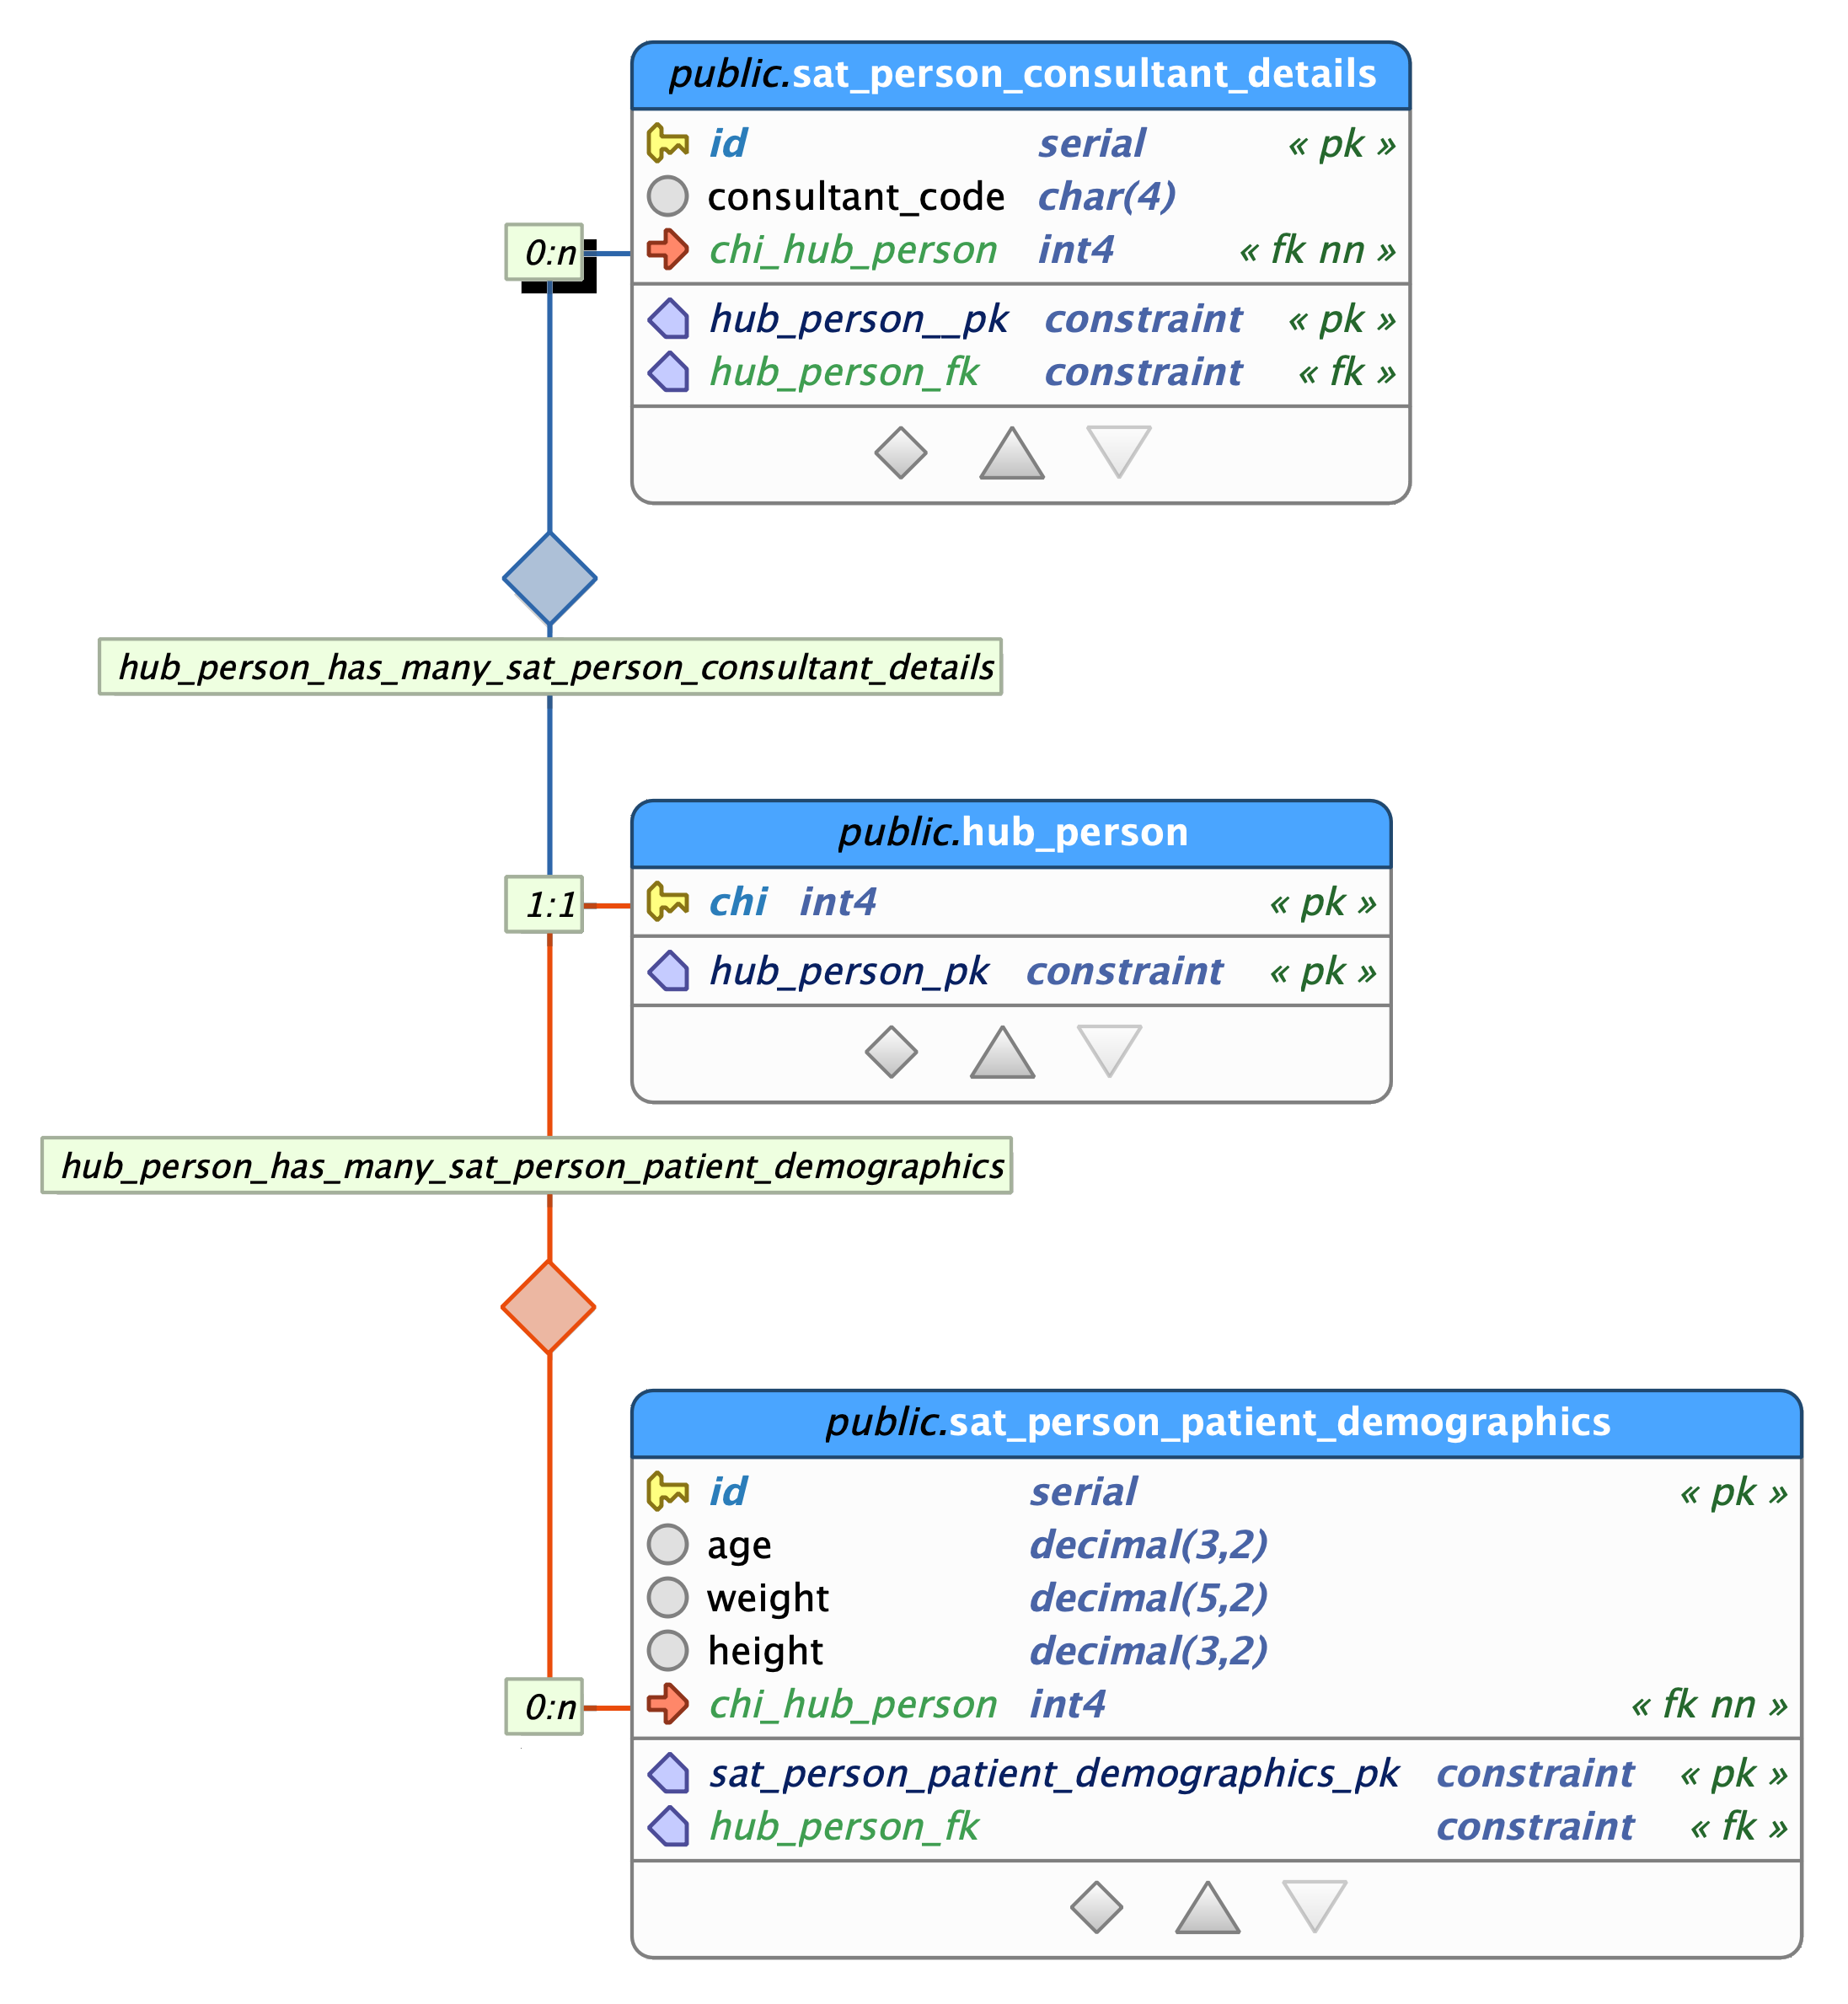
\includegraphics[width=10cm]{figures/technical/satellites.png}
    \caption{Data Vault - T-P-O-L-E Satellites}
    \label{fig:dvsatellites}
\end{figure}
\end{itemize}



\section{Reference tables}

Reference tables are a normal part of a healthy data vault model. These will hold look-ups and standards for common codes within the complete data vault.

This is the area where the standards are stored ready for the data vault to use during the upload.

\section{What is a T-P-O-L-E Data Vault?}

The Time-Person-Object-Location-Event (T-P-O-L-E) Data Vault is a highly specific data vault that reduces all business activities to be generalised as one of five types of hubs.

The hubs are:
\begin{itemize}
    \item Time Hub
    The time is sub-divided as Date and Time.
    Prescribes ISO 8601-1:2019 and ISO 8601-2:2019 as standards.
    
    \item Person Hub
    The person involve is record using concept of "Golden Nominal"
    This type of record is a single person record with a unique reference proven to that single person.
    
    \item Object Hub
    The objects are any other referable entities involved in the interaction.
    Examples are:
    \begin{itemize}
        \item Organisations (Legal entity of Bank, Hospital or School)
        \item Physical objects (Bank Card, Vehicle or hospital bed)
        \item Buildings (Physical Bank, Hospital or School)
    \end{itemize}
    \item Location Hub
    The location is to one thousandth of a latitude and longitude (i.e. to less than one square meter) using ISO 6709:2008 Standard. (\url{https://www.iso.org/standard/39242.html})
    
    Note that the location stores different descriptions via location satellites for the same location.
    
    Example: a location could be a building's location, physical address and a bus stop on a bus route at the same time.
    
    \item Event Hub
    The event is the individual action or event recorded.
    
\end{itemize}

The links are force to be only between these T-P-O-L-E hubs to limit the complexity of the core structure of the model. These links are different for each implementation of the T-P-O-L-E methodology but is high descriptive via meta-data how and what is stored in the links.

The satellites are connected to T-P-O-L-E hubs to add the temporal attributes and descriptive attributes.
These satellites holds all the attributes for a specific type of hub.
These common attributes between satellites are the concept that the specific values was valid from a specific point in time until another point in time.

Note: Data is never delete or modified as it is immutable. All transactions are inserts to indicate the latest state of the data. This creates a complete history with provenance and full lineage.



\section{Smart Patient Electronic Health Record - Cancer.Informatics}

(See: Cancer.Informatics Use Case \ref{chap:usecase})

\section{Use Case Description}

(See: Cancer.Informatics Use Case Description \ref{sec:usecasecancer})

\section{Entity Relationship Diagram (ERD) - Cancer.Informatics}

This Entity Relationship Diagram (ERD) shows the details for the first source system from University of St Andrews the team use to show how the sources system is stored in its native form in the health care ecosystem.

\begin{figure}[H]
    \centering
    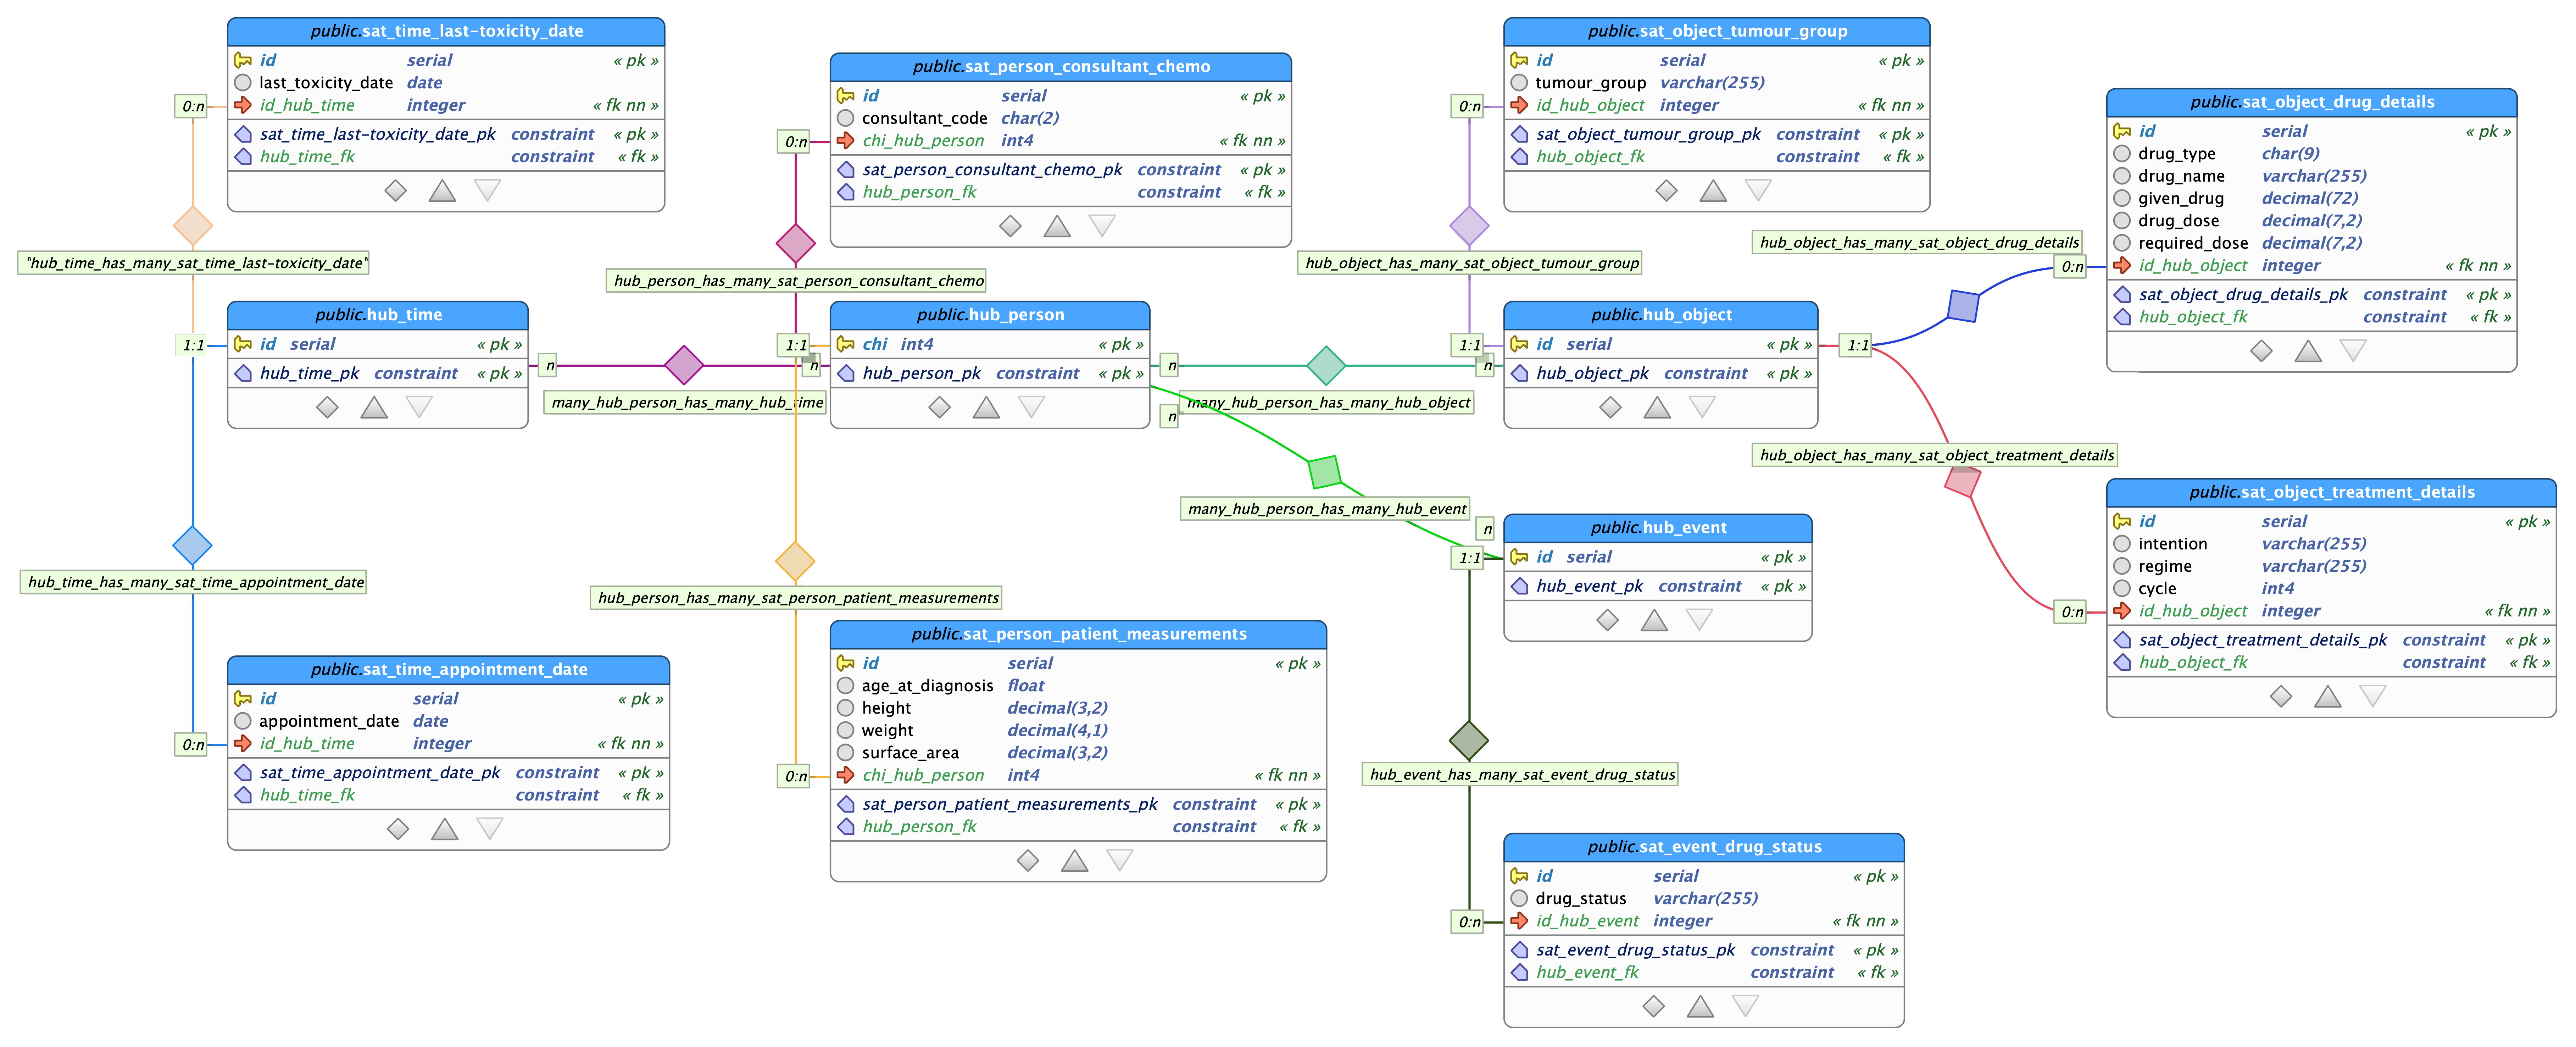
\includegraphics[width=14cm]{figures/technical/dv_chemocare_treatment_db.png}
    \caption{ERD - Cancer.Informatics}
    \label{fig:figERD_CancerInformatics}
\end{figure}

\section{Hierarchical Data Format version 5 (HDF5)}

Hierarchical Data Format (HDF) is a set of file formats of which HDF5 is the version 5. It is design with basic principals to store and organise large amounts of data. \ref{fig:figHDF5} \cite{Folk2011}

\begin{figure}[H]
    \centering
    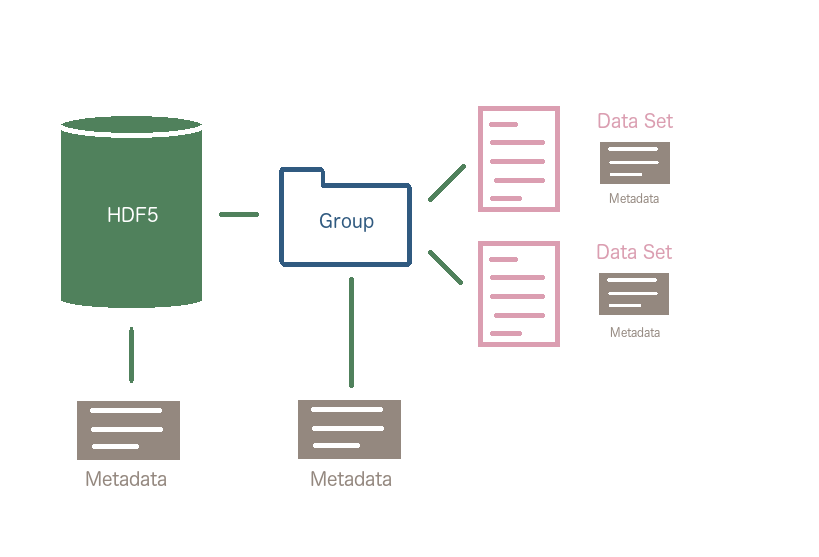
\includegraphics[width=10cm]{figures/technical/HDF5.png}
    \caption{Hierarchical Data Format (HDF) version 5}
    \label{fig:figHDF5}
\end{figure}

The research project is using a \href{https://pypi.org/project/h5py/}{H5Py} library to build and maintain the data.

The record is structured using HDF groups that supports the core hubs of the data vault.

These hubs are:

\begin{itemize}
    \item Time
    
    The project support ISO 8601-1:2019 (\url{https://www.iso.org/obp/ui#iso:std:iso:8601:-1:ed-1:v1:en})
    and ISO 8601-2:2019 Notation 
    (\url{https://www.iso.org/obp/ui#iso:std:iso:8601:-2:ed-1:v1:en})
    for date format. \\
    Datetime with time zone (yyyy-mm-ddThh:mm:ss.nnnnnn+|-hh:mm)
    
    
    \item Person
    Core information on the persons involve in the health-care process.
    These can be patient, medical staff or other authorised persons.
    The role of the person is determine by a person role type in the hub.
    
    \item Object
    Core information on the objects involve in the health-care process.
    These can be blood samples, hospital beds etc.
    The role of the object is determine by a object role type in the hub.
    
    \item Location
    Core information on the locations involve in the health-care process.
    Project supports ISO 6709:2008 Standard. (\url{https://www.iso.org/standard/39242.html})
    
    
    The location is to one thousandth of a latitude and longitude (i.e. to less than one square meter).
    The role of the location is determine by a location role type in the hub.
    Suggestion currently is a single type: latitude-longitude.
    
    \item Event
    Core information on the events involve in the health-care process.
    The role of the event is determine by a event role type in the hub.
    Examples of events:
    \begin{itemize}
        \item Patient visit to doctor.
        \item Patient takes medical test.
        \item Patient performs Physiotherapy exercise with sensors attached.
        \item Patient answer Prompts on Quality of Life question.
    \end{itemize}
    
    
\end{itemize}

\begin{figure}[H]
    \centering
    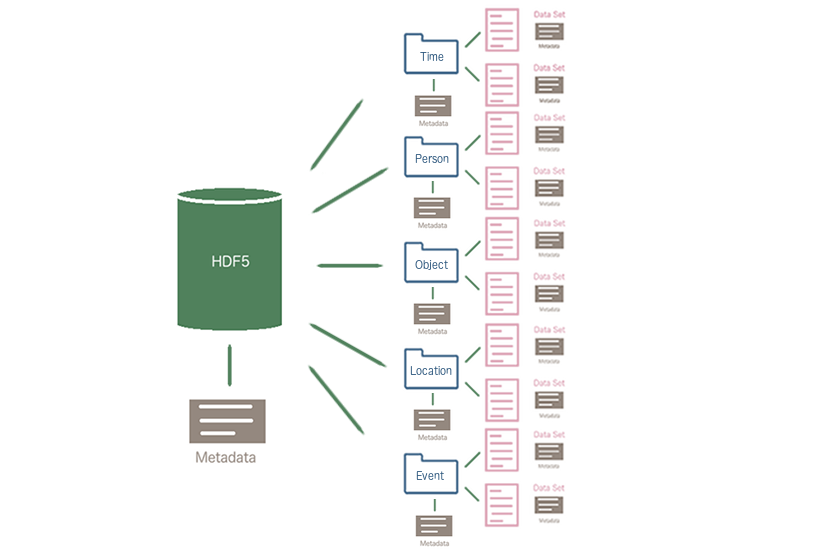
\includegraphics[width=14cm]{figures/technical/HDF5_TPOLE.png}
    \caption{T-P-O-L-E HDF version 1.00}
    \label{fig:figHDF5TPOLE}
\end{figure}